%%Section4-5

\section{実験装置}
\begin{figure}[h]
  \begin{center}
    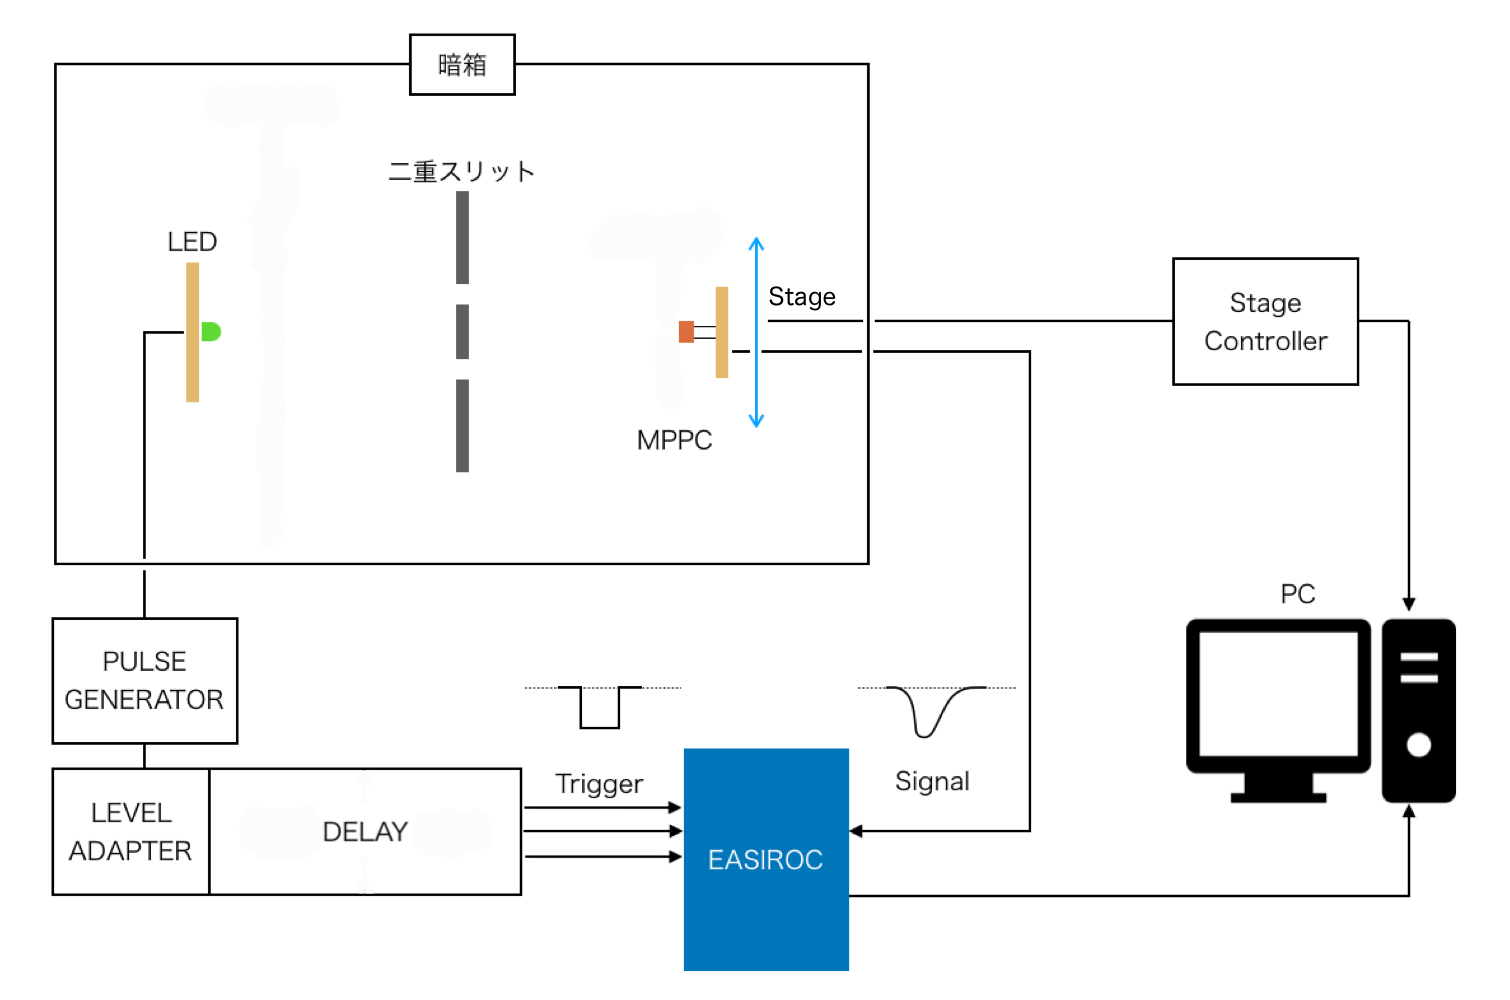
\includegraphics[width=12cm]{../setup_2021.jpeg}
  \end{center}
  \caption{実験の模式図}
\end{figure}

本実験で用いる実験装置.
\begin{itemize}
  \item 光源(LED)
  \item 光検出器(MPPC)
  \item MPPC読み出しモジュール(EASIROC)
  \item 二重スリット
  \item 可動式ステージ\par
        「Stage Controller」で制御.MPPCが設置されている基盤の位置を可動式ステージで細かく変更することが可能.
  \item 波高発生器(PULSE GENERATOR)\par
        非常に高い(1kHz)周期で矩形波を出力.出力と同期してトリガーを出力することも可能.
  \item レベルアダプター(LEVEL ADAOTER)\par
        TTL 入力信号をNIM 信号に変換し, 出力.
  \item 遅延回路(DELAY)\par
        信号を遅らせるもの.要は長いケーブル.
  \item 測定用PC \par
        EASIROCの制御や, 可動式ステージの制御を行う.データ取得まで行うことができる.
\end{itemize}
光学機器を図のように並べ, 光の干渉を起こす.各デバイスの位置や距離によって干渉の見え方が変わるが, これは実際に物を置いていろいろ試してみるとよい.以下では, 光検出器とその読み出しについて説明する.

\subsection{光検出器}
光センサにはたくさんの種類があるが、どれも光を電気信号に変換して取り出すという点は共通している。
今回の実験で用いるのはMPPCと呼ばれる優れた光子カウント能力を持つ小型の光検出器である。

\subsubsection{半導体}
半導体の電気伝導度は金属と絶縁体の中間の値をとり、温度、光、および微量の不純物に対し非常に敏感である。
エネルギーバンドを考えると、金属は伝導帯が部分的に電子に占有されているか、価電子帯と重なっているかなため、バンドギャップがない。したがって、電子はわずかな外部電場によって自由に移動できる。
絶縁体では、荷電しは隣接原子間の強い結合を担っているため、室温付近では電気伝導に寄与する自由電子は存在しない。伝導帯は空で、バンドギャップは$\sim9$eVである。
半導体のエネルギーギャップは1eV程度で、0Kではすべての電子は価電子帯にあり伝導帯は空である。室温(かつ通常の圧力)では、エネルギーギャップは室温の熱エネルギー$k_BT$の数十倍であり、かなりの数の電子が価電子帯から伝導帯へ熱的に励起される。
伝導帯には多くの殻の電子状態があるため、わずかな電場でこれらの電子を移動させることができる。
不純物の数が熱的に励起された電子正孔の数より少ない半導体を真性半導体という。GeやSiがあるが、室温動作に優れ、高品質のSiO2が熱酸化で形成できること、また地殻の25\%を占めることから、Siデバイスが実用的に使われている。
真性半導体では伝導帯の電子密度と価電子帯の正孔密度は等しい。
半導体に不純物をドープすると、不純物準位が生じる。
Si原子が価電子5の原子(例えばAs)に置換されるとn型半導体、価電子3の原子(例えばB)に置換されるとp型半導体になる。ここでAsをドナー、Bをアクセプタという。
n型半導体の多数キャリアは電子(少数キャリアは正孔)、p型半導体の多数キャリアは正孔(少数キャリアは電子)である。

\subsubsection{pn接合}


\subsubsection{なだれ(アバランシェ)増幅}
量子トンネル効果により、ポテンシャル障壁を通り抜けて左側の半導体から右側の半導体に移動することで、逆バイアスで電流が流れることがある。

\subsubsection{MPPC}
MPPC(Micro Pixel Photon Counter)はAvalamche Photo Diode(APD)が多数配列された光検出器である.APDは半導体でできている.
P型とN型, 異なるドープ型の半導体にある向きで電圧をかけると, キャリアの少ない空乏層ができる.
ここに光子が入射すると, 光電効果で電子をはじき出す.
電子は印加電圧によってエネルギーを持ち, さらに周囲の原子殻内電子をはじき出し, 雪崩(Avalanche)的に電子を倍増する.
印加電圧によって様々な倍増モードがあるが, MPPC内のAPDでは, 十分な印加電圧をかけることで入射光子数によらない出力電流を得る(ガイガーモード).
このガイガーモードAPDが多数配列することにより, 我々は光子が入射したAPDのチャンネル数だけを数えることで, (pile upはあるものの)光子数をデジタルに数えることができる.
\begin{figure}[h]
  \begin{tabular}{ccc}
    \begin{minipage}[t]{0.33\hsize}
      \begin{center}
        \includegraphics[width=4cm]{../mppc.jpg}
      \end{center}
      \caption{MPPC}
    \end{minipage}
    \begin{minipage}[t]{0.33\hsize}
      \begin{center}
        \includegraphics[width=4cm]{../APDstructure.PNG}
      \end{center}
      \caption{APD}
    \end{minipage}
    \begin{minipage}[t]{0.33\hsize}
      \begin{center}
        \includegraphics[width=4cm]{../QuenchingArray.PNG}
      \end{center}
      \caption{MPPCはAPDを並列に並べたもの}
    \end{minipage}
  \end{tabular}
\end{figure}

浜松ホトニクスのハンドブックに, 詳細なMPPCの挙動が説明されている.\cite{hamamatsu}

\subsection{EASIROC}
EASIROCモジュールは, 書き換え不可能な集積回路(ASIC)であるEASIROCチップと, EASIROCチップ制御用の書き換え可能な集積回路(FPGA)であるArtix7が搭載された, MPPCの(多チャンネネル)読み出しモジュールである.今回は1チャンネルしか使わないし, FPGAのfirmwareの書き換えも(おそらく)ないので, ここでは, EASIROCチップの回路の概要と, アナログな出力波形について見ることにする.\\
EASIROCチップは, Pre-Amp,Shaper,Discriminator,Capacitorからなる.Pre-Amp,Slow Shaperを通った信号電圧をCapacitorに保存し, Trigger信号が入力されたときに電圧をholdし, ADC(Analog Digital Converter)でデジタル情報に変換する.
\begin{figure}[H]
  \begin{center}
    \includegraphics[width=12cm]{../EASIROCCircuitDiagram.PNG}
  \end{center}
  \caption{EASIROC回路概略}
\end{figure}

\begin{figure}[H]
  \begin{tabular}{cccc}
    \begin{minipage}[t]{0.25\hsize}
      \begin{center}
        \includegraphics[width=4cm]{../preamp.BMP}
      \end{center}
      \caption{Pre-Amp}
    \end{minipage}
    \begin{minipage}[t]{0.25\hsize}
      \begin{center}
        \includegraphics[width=4cm]{../fastshaper.BMP}
      \end{center}
      \caption{Fast Shaper}
    \end{minipage}
    \begin{minipage}[t]{0.25\hsize}
      \begin{center}
        \includegraphics[width=4cm]{../slowshaper.BMP}
      \end{center}
      \caption{Slow Shaper}
    \end{minipage}
    \begin{minipage}[t]{0.25\hsize}
      \begin{center}
        \includegraphics[width=4cm]{../slowshaperhold.BMP}
      \end{center}
      \caption{holdしたSlow Shaper}
    \end{minipage}
  \end{tabular}
\end{figure}


各デバイスを通った信号の出力波形は, EASIROCモジュールのProbe出力を観察するとわかる.Fast ShaperはSelf Trigger用なので, 今回は(おそらく)使わない.Trigger信号に合わせてShaperの波高の一番高いところが読み出されているのがわかる.Trigger信号とShaperの立ち上がりがきちんと合うかどうかはケーブルの長さやDelayモジュールによって操作できる.

\section{測定方法}

\subsection{可動式ステージの使用方法}

可動式ステージは, stage.pyを用いて制御する.使用するためのコマンドは, 以下の通りである.
\begin{figure}[H]
  \begin{lstlisting}[caption=stage.pyのコマンド]
$ ./stage.py [コマンド]  
  \end{lstlisting}
\end{figure}


\begin{table}[H]
  \begin{center}
    \caption{stage.py コマンド一覧}
    \begin{tabular}{|l|l|l|} \hline
      入力コマンド & 使い方       & 動作                                      \\ \hline \hline
      -o           & -o           & left or right 側の原点に戻る              \\ \hline
      -r           & -r           & データリセット, 現在地を原点とする        \\ \hline
      -mr          & -mr [整数値] & 今いるところから[整数値]パルス分+側へ移動 \\ \hline
      -ml          & -ml [整数値] & 今いるところから[整数値]パルス分-側へ移動 \\ \hline
      -pr          & -pr [整数値] & 絶対的な座標位置+[整数値]パルスへ移動     \\ \hline
      -pl          & -pl [整数値] & 絶対的な座標位置-[整数値]パルスへ移動     \\ \hline
      -s           & -s           & 動作停止                                  \\ \hline
      -q           & -q           & ステージの情報を表示                      \\ \hline
      -h           & -h           & コマンドの使い方表示                      \\ \hline
    \end{tabular}
  \end{center}
\end{table}

\begin{itembox}[l]{注意事項}
  \begin{itemize}
    \item 動く距離とパルスの関係は2μm/パルス.
    \item 一度の操作で送ることのできるコマンドは1つ.
    \item 複数送った場合, コマンド一覧の上から順に優先順位がついており, 優先順位が最も高いものの動作を行う.
  \end{itemize}
  例えば, {\tt \$ ./stage.py -ml 1000 -mr 20000 -s -o +} とコマンドを送っても, {\tt -o} のみが認識される.
\end{itembox}


\subsection{EASOROCの使用方法}

\subsubsection{EASIROCモジュールへのアクセス}
\begin{lstlisting}
$ ./Controller.rb 192.168.10.102
\end{lstlisting}
でEASIROCモジュールとのシェル上での対話が可能になる.
利用できる主なコマンドは表\ref{table:easiroc_controller_commands}の通りである.
詳しい情報は\href{https://ppwww.phys.sci.kobe-u.ac.jp/~hamada/easiroc_manual.html}{ここのリンク}を参照.

\begin{table}[htbp]
  \begin{center}
    \caption{easiroc コマンド一覧}
    \label{table:easiroc_controller_commands}
    \begin{tabular}{|l|l|} \hline
      入力コマンド & 動作                                                     \\ \hline \hline
      setHV [bias voltage] & HVを[bias voltage]の値にセットする\\ \hline
      statusHV & HVの電圧と電流を表示する\\ \hline
      read [EventNum] [Filename] & データ取得を行う \\ \hline
      exit, quit & プログラムの終了\\ \hline
    \end{tabular}
  \end{center}
\end{table}

\subsubsection{印加電圧の設定}

たとえば, コントローラを起動したシェルで
\begin{lstlisting}
$ setHV 10
\end{lstlisting}
を実行することでMPPCにバイアス電圧10Vが印加される.
setHVコマンドの実行後は
\begin{lstlisting}
$ statusHV
\end{lstlisting}
を用いてMPPCにかかっている実際のバイアス電圧と電流を確認すること.
光漏れなどの原因によりMPPCに異常な電流が流れていないかを確認することが主な目的である.

\begin{itembox}[l]{注意事項}
  \begin{itemize}
    \item 電流は正常な値で数$\mathrm{\mu A}$程度である.10 倍以上の電流が流れるようであればすぐにsetHV 0 を実行し, 大電流が流れた原因を考えること
  \end{itemize}
\end{itembox}

\subsubsection{EASIROC測定手順}
\begin{itemize}
  \item Controller.rbを用いてEasirocに接続
  \item HG outからの出力をみながら電圧を設定
  \item readコマンドを打って測定開始
\end{itemize}
測定データはController.rbがあるディレクトリ配下のdataディレクトリ以下に保存される.
測定データの確認方法は以下の通りである.
\begin{lstlisting}
$ cd data
$ root filename.root
$ TBrowser t
\end{lstlisting}
または
\begin{lstlisting}
$ cd data
$ root filename.root
$ ADC_HIGH_12->Draw()
\end{lstlisting}
